The single asset test cases are designed to test the basic elements of the event-based risk calculator, such as:

\begin{itemize}
\item asset event loss table computation
\item asset loss exceedance curve computation
\end{itemize}

The location and taxonomy of the single asset in the exposure model used for the single-asset test cases for the event-based risk calculator are given in Table \ref{tab:asset}.

% ---------------------------------------------------------------------------
\subsubsection{Case 1a}
The source model used for this test case comprises a simple vertical strike-slip fault using a truncated Gutenberg-Richter magnitude-frequency distribution.\\

\noindent Details of the source model are listed below:\\

\noindent
Fault type: Strike slip\\
Fault dip: $90^{\circ}$\\
Fault plane depths: 0--12 km\\
Fault coordinates:\\
South end: $38.0000^{\circ} N$, $122.0000^{\circ} W$\\
North end: $38.2248^{\circ} N$, $122.0000^{\circ} W$\\
Rupture aspect ratio: 2.0\\
Rake angle: $0^{\circ}$\\
Magnitude scaling relationship: Wells and Coppersmith (1994)\\
Magnitude-frequency distribution:\\
Truncated Gutenberg-Richter: $a = 3.1292; b = 0.9; M_{min} = 5.0; M_{max} = 6.5$\\

The time period for both the hazard and the risk calculations in this case are one year. This case uses a collection of 100,000 stochastic event sets, each spanning one year, to generate a set of ground motion fields representative of the seismicity of the specified region, collectively spanning a period of 100,000 years. A single stochastic event set (SES) may contain zero or more ruptures that are generated based on the frequency distribution of the sources. Each SES in this case represents one simulation of the possible events that might occur in one year.

Table~\ref{tab:vf-ln-tax1-zcov} shows the mean loss ratios and corresponding coefficients of variation in the lognormal vulnerability function used in this case. There is no uncertainty in the vulnerability function used for this case. The coefficient of variation of the loss ratio is zero at all intensity measure levels. The purpose of this case is to test the correct interpolation of the mean loss ratios of the vulnerability function at intermediate intensity measure levels and verify the steps involved in the computation of the asset loss exceedance curve and average annual loss.

The hazard calculation produces 4,115 ruptures over the 100,000 cumulative time span, and 4,115 corresponding ground motion fields. The ground motion values at the location of the single asset are $[0.074, 0.154, 0.118, 0.203, \dots, 0.288] g$ (4,115 ground motion values in total).

The calculation of the loss ratios given the ground motion values proceeds in exactly the same manner as described in the Scenario Risk calculator examples. The mean loss ratio and coefficient of variation of the loss ratio are obtained by linear interpolation from the provided vulnerability model for each of the above 4,115 ground motion values. Finally, a loss ratio is sampled from the lognormal distribution defined by the interpolated mean and standard deviation parameters for each ground motion value. Particularly in this case, since there is no variability in the loss ratio, calculation of the loss ratios for each ground motion field is straightforward in this case. Since the coefficients of variation in the vulnerability function are all zero, the lognormal distribution devolves into the degenerate distribution.

These numbers are multiplied by the asset value of $10,000$ to give 4,115 sampled loss values: $[148.90, 308.60, 236.14, 408.76, \dots, 665.79]$ (4,115 loss values in total). This set of losses forms the event loss table (ELT) for the asset.

For the computation of the asset loss curve, the range of loss spanning the minimum and maximum loss observed in the ELT is divided into a number of equispaced intervals as specified by the parameter `loss\_curve\_resolution'. In this case, a value of ten is used for the `loss\_curve\_resolution' parameter. The maximum loss observed in the ELT is $9,713.29$, and the minimum loss observed is $0$. The loss curve is thus calculated at the following eleven points: $[0.00, 1079.25, 2158.51, 3237.76, 4317.02, 5396.27, 6475.53, 7554.78, 8634.03, 9713.29]$.

At each of the eleven loss values on the loss curve, the annual frequency of exceedance of that loss value is obtained by counting the number of ruptures in the ELT which produce losses greater than that loss value, and dividing the count by the cumulative time span of 100,000 years. The loss exceedance counts for the eleven loss values shown above are: $[4030, 799, 293, 133, 87, 48, 25, 13, 6, 0]$. Dividing these exceedance counts by 100,000 gives the corresponding annual exceedance rates or frequencies: $[4.030\times10^{-2}, 7.990\times10^{-3}, 2.930\times10^{-3}, 1.330\times10^{-3}, 8.700\times10^{-4}, 4.800\times10^{-4}, 2.500\times10^{-4}, 1.300\times10^{-4}, 6.000\times10^{-5}, 0.000]$.

Finally, the probabilities of exceedance for the set of eleven loss values are calculated from the annual frequencies of exceedance $\lambda_{L \geq l}$ and the exposure time period $t_R$ through:

\begin{equation}
	prob(L \geq l, t_R) = 1 - \exp (-\lambda_{L \geq l} \times t_R)
\end{equation}

The probabilities of exceedance for the eleven loss values are computed to be the following: $[3.950\times10^{-2}, 7.958\times10^{-3}, 2.926\times10^{-3}, 1.329\times10^{-3}, 8.696\times10^{-4}, 4.799\times10^{-4}, 2.500\times10^{-4}, 1.300\times10^{-4}, 6.000\times10^{-5}, 0.000]$.

The loss curve thus calculated above using the implementation of the calculator in Julia is compared with the loss curve obtained using the OpenQuake classical PSHA based risk calculator in Figure~\ref{fig:lc-ebr-1a}.

\begin{figure}[htbp]
\centering
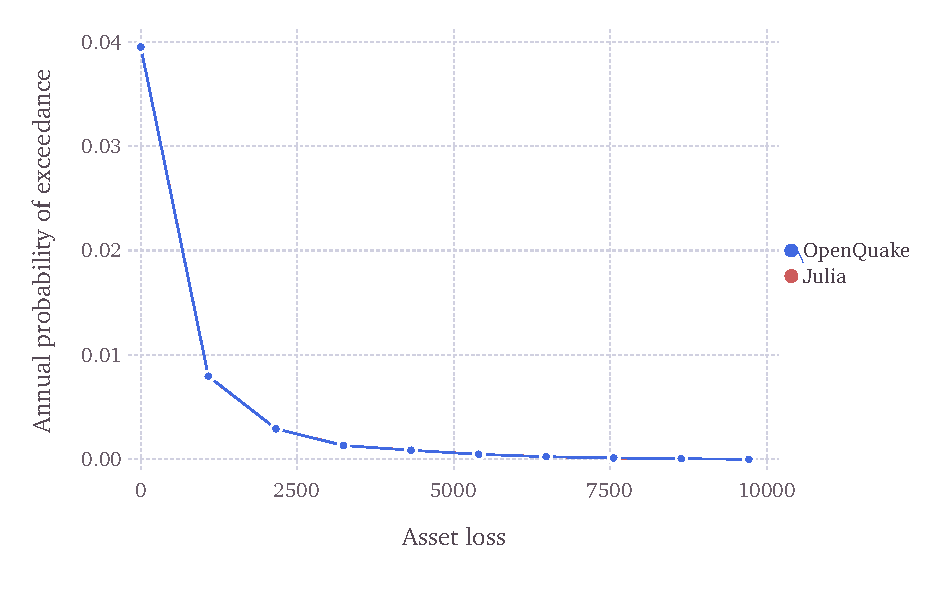
\includegraphics[width=12cm]{qareport/figures/fig-lc-ebr-1a}
\caption{Loss curve comparison for event based risk test case 1a}
\label{fig:lc-ebr-1a}
\end{figure}

The area under the annual loss exceedance curve gives the average annual loss.
\begin{table}[htbp]

\centering
\begin{tabular}{ l r r r }

\hline
\rowcolor{anti-flashwhite}
\bf{Result} & \bf{Expected} & \bf{OpenQuake} & \bf{Difference}\\
\hline
Average loss & 36.43 & 36.43 & 0.00\% \\
\hline
\end{tabular}

\caption{Results for event based risk test case 1a}
\label{tab:result-ebr-1a}
\end{table}
Table \ref{tab:result-ebr-1a} shows the comparison of the OpenQuake result for average annual loss with the expected result.

% ---------------------------------------------------------------------------
\subsubsection{Case 1b}
The time period for both the hazard and the risk calculations in this case are one year. This case uses a collection of 100,000 stochastic event sets, each spanning one year, to generate a set of ground motion fields representative of the seismicity of the specified region, collectively spanning a period of 100,000 years. A single stochastic event set (SES) may contain zero or more ruptures that are generated based on the frequency distribution of the sources. Each SES in this case represents one simulation of the possible events that might occur in one year.

Table~\ref{tab:vf-ln-tax1-zcov} shows the mean loss ratios and corresponding coefficients of variation in the lognormal vulnerability function used in this case. There is no uncertainty in the vulnerability function used for this case. The coefficient of variation of the loss ratio is zero at all intensity measure levels. The purpose of this case is to test the correct interpolation of the mean loss ratios of the vulnerability function at intermediate intensity measure levels.

Since there is no variability in the loss ratio, calculation of the loss ratios for each ground motion field is straightforward in this case. Since the coefficients of variation in the vulnerability function are all zero, the lognormal distribution devolves into the degenerate distribution. The hazard calculation produces 4,115 ruptures over the 100,000 cumulative time span, and 4,115 corresponding ground motion fields. The ground motion values at the location of the single asset are $[0.074, 0.154, 0.118, 0.203, \dots, 0.288] g$ (4,115 values in total).

The calculation of the loss ratios given the ground motion values proceeds in exactly the same manner as described in the Scenario Risk calculator examples. The mean loss ratio and coefficient of variation of the loss ratio are obtained by linear interpolation from the provided vulnerability model for each of the above 4,115 ground motion values. Finally, a loss ratio is sampled from the lognormal distribution defined by the interpolated mean and standard deviation parameters for each ground motion value.

These numbers are multiplied by the asset value of $10,000$ to give 4,115 sampled loss values.
\begin{table}[htbp]

\centering
\begin{tabular}{ l r r r }

\hline
\rowcolor{anti-flashwhite}
\bf{Result} & \bf{Expected} & \bf{OpenQuake} & \bf{Difference}\\
\hline
Average loss & 139.14 & 139.14 & 0.00\% \\
\hline
\end{tabular}

\caption{Results for event based risk test case 1b}
\label{tab:result-ebr-1b}
\end{table}
Table \ref{tab:result-ebr-1b} shows the comparison of the OpenQuake result for average annual loss with the expected result.

% ---------------------------------------------------------------------------
\subsubsection{Case 1c}
The source model used for this test case comprises a characteristic fault.\\

\noindent Details of the source model are listed below:\\

\noindent
Fault type: Strike slip\\
Fault dip: $30^{\circ}$\\
Fault plane depths: 5--15 km\\
Fault coordinates:\\
$38.0000^{\circ} N$, $122.4000^{\circ} W$\\
$38.2248^{\circ} N$, $122.0000^{\circ} W$\\
$38.2248^{\circ} N$, $121.7000^{\circ} W$\\
Rake angle: $0^{\circ}$\\
Magnitude-frequency distribution:\\
Characteristic: $M = 7.0$; bin width = $0.1$; occurance rate = $0.04$\\

Apart from the different source model, this case is similar to Case~1a, and once again, is only included here as the numbers from this case will be useful in later cases involving a nontrivial source model logic tree with more than branch. The loss curve calculated using the implementation of the calculator in Julia is compared with that produced by OpenQuake in Figure~\ref{fig:lc-ebr-1c}.

\begin{figure}[htbp]
\centering
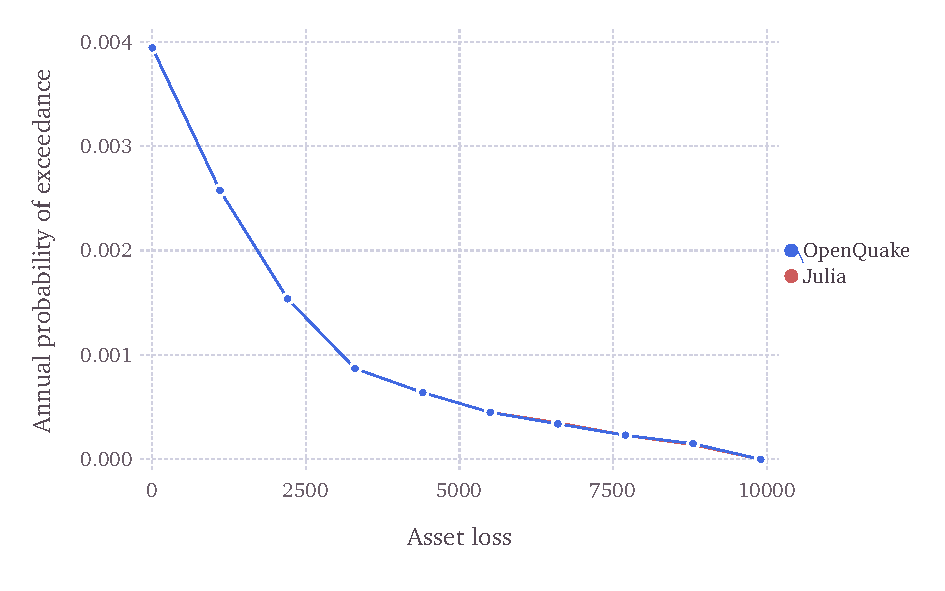
\includegraphics[width=12cm]{qareport/figures/fig-lc-ebr-1c}
\caption{Loss curve comparison for event based risk test case 1c}
\label{fig:lc-ebr-1c}
\end{figure}

The area under the annual loss exceedance curve gives the average annual loss.
\begin{table}[htbp]

\centering
\begin{tabular}{ l r r r }

\hline
\rowcolor{anti-flashwhite}
\bf{Result} & \bf{Expected} & \bf{OpenQuake} & \bf{Difference}\\
\hline
Average loss & 9.64 & 9.64 & 0.00\% \\
\hline
\end{tabular}

\caption{Results for event based risk test case 1c}
\label{tab:result-ebr-1c}
\end{table}
Table \ref{tab:result-ebr-1c} shows the comparison of the OpenQuake result for average annual loss with the expected result.
% ---------------------------------------------------------------------------
\subsubsection{Case 1d}
The purpose of this case is to test the loss ratio sampling when the lognormal vulnerability model has nonzero coefficients of variation of the loss ratios. Table~\ref{tab:vf-ln-tax1-nzcov} shows the mean loss ratios and corresponding coefficients of variation in the vulnerability model used in this test case.

Apart from the nonzero coefficients of variation in the vulnerability model, this case is similar to Case~1a. The only difference enters during the loss ratio sampling stage, where the lognormal distribution no longer devolves into the degenerate distribution.

As in Case~1a, the mean loss ratio and coefficient of variation of the loss ratio are obtained by linear interpolation from the provided vulnerability model for each of the 4,115 ground motion values produced by the hazard calculation. A loss ratio is now sampled from the lognormal distribution defined by the interpolated mean and standard deviation parameters for each ground motion value. The rest of the calculation steps involved in the computation of the event loss table, loss exceedance curve, and average annual loss remain the same as described in Case~1a.

The loss curve calculated using the implementation of the calculator in Julia is compared with that produced by OpenQuake in Figure~\ref{fig:lc-ebr-1d}.

\begin{figure}[htbp]
\centering
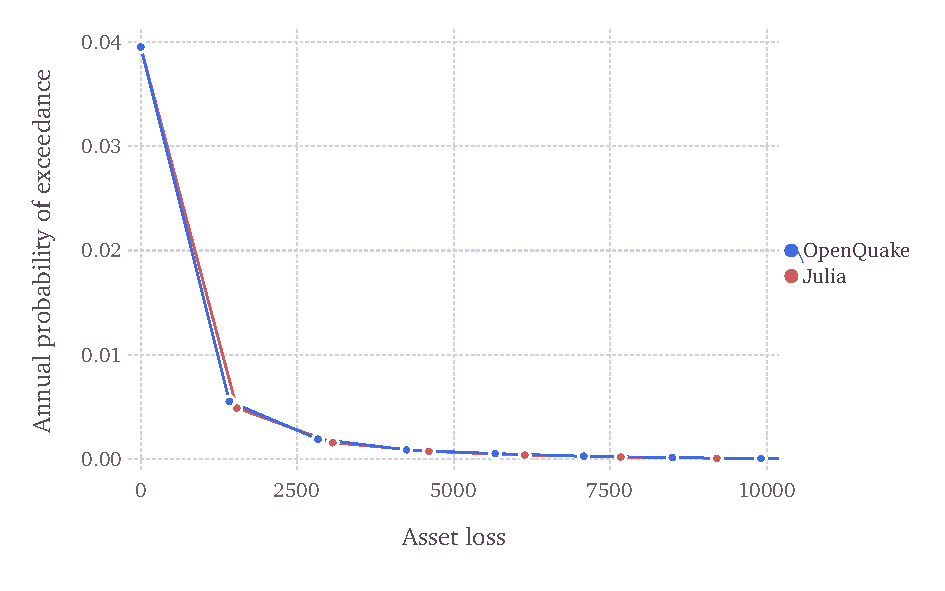
\includegraphics[width=12cm]{qareport/figures/fig-lc-ebr-1d}
\caption{Loss curve comparison for event based risk test case 1d}
\label{fig:lc-ebr-1d}
\end{figure}

The area under the annual loss exceedance curve gives the average annual loss.
\begin{table}[htbp]

\centering
\begin{tabular}{ l r r r }

\hline
\rowcolor{anti-flashwhite}
\bf{Result} & \bf{Julia} & \bf{OpenQuake} & \bf{Difference}\\
\hline
Average loss & 42.60 & 46.18 & 8.06\% \\
\hline
\end{tabular}

\caption{Results for event based risk test case 1d}
\label{tab:result-ebr-1d}
\end{table}
Table \ref{tab:result-ebr-1d} shows the comparison of the OpenQuake result for average annual loss with the expected result.

% ---------------------------------------------------------------------------
\subsubsection{Case 1e}
This test case is identical to Case~1a described above, except for the use of the Beta distribution for the vulnerability functions instead of the lognormal distribution. Since the coefficients of variation in the vulnerability function are all zero, once again the Beta distribution devolves into the degenerate distribution as in Case~1a. The results for this test case should be exactly the same as in Case~1a.

The loss curve calculated using the implementation of the calculator in Julia is compared with that produced by OpenQuake in Figure~\ref{fig:lc-ebr-1e}.

\begin{figure}[htbp]
\centering
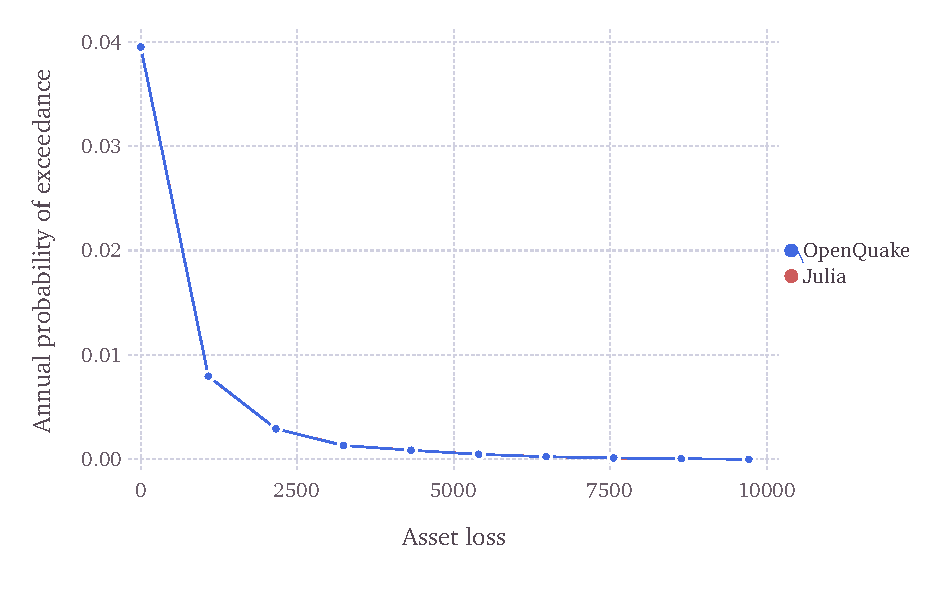
\includegraphics[width=12cm]{qareport/figures/fig-lc-ebr-1e}
\caption{Loss curve comparison for event based risk test case 1e}
\label{fig:lc-ebr-1e}
\end{figure}

The area under the annual loss exceedance curve gives the average annual loss.
\begin{table}[htbp]

\centering
\begin{tabular}{ l r r r }

\hline
\rowcolor{anti-flashwhite}
\bf{Result} & \bf{Expected} & \bf{OpenQuake} & \bf{Difference}\\
\hline
Average loss & 36.43 & 36.43 & 0.00\% \\
\hline
\end{tabular}

\caption{Results for event based risk test case 1e}
\label{tab:result-ebr-1e}
\end{table}
Table \ref{tab:result-ebr-1e} shows the comparison of the OpenQuake result for average annual loss with the expected result.

% ---------------------------------------------------------------------------
\subsubsection{Case 1f}
The purpose of this case is to test the loss ratio sampling when the Beta vulnerability model has nonzero coefficients of variation of the loss ratios. Table~\ref{tab:vf-ln-tax1-nzcov} shows the mean loss ratios and corresponding coefficients of variation in the vulnerability model used in this test case.

Apart from the nonzero coefficients of variation in the vulnerability model, this case is similar to Case~1e. The only difference enters during the loss ratio sampling stage, where the Beta distribution no longer devolves into the degenerate distribution.

The loss curve calculated using the implementation of the calculator in Julia is compared with that produced by OpenQuake in Figure~\ref{fig:lc-ebr-1f}.

\begin{figure}[htbp]
\centering
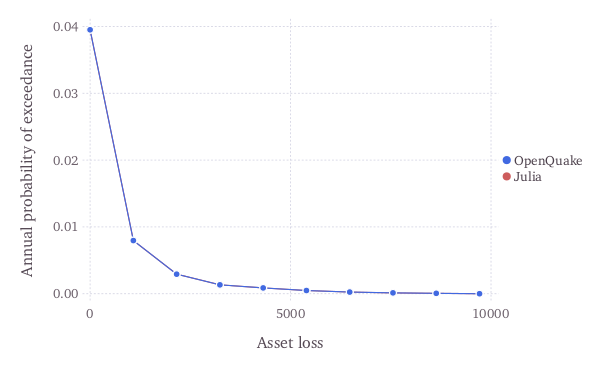
\includegraphics[width=12cm]{qareport/figures/fig-lc-ebr-1f}
\caption{Loss curve comparison for event based risk test case 1f}
\label{fig:lc-ebr-1f}
\end{figure}

The area under the annual loss exceedance curve gives the average annual loss.
\begin{table}[htbp]

\centering
\begin{tabular}{ l r r r }

\hline
\rowcolor{anti-flashwhite}
\bf{Result} & \bf{Expected} & \bf{OpenQuake} & \bf{Difference}\\
\hline
Average loss & 36.80 &  & \% \\
\hline
\end{tabular}

\caption{Results for event based risk test case 1f}
\label{tab:result-ebr-1f}
\end{table}
Table \ref{tab:result-ebr-1f} shows the comparison of the OpenQuake result for average annual loss with the expected result.

% ---------------------------------------------------------------------------
\subsubsection{Case 1g}
This test case repeats the exercise from Case~1d and Case~1f, using the discrete probability vulnerability functions instead of the parametric lognormal or Beta distribution based functions used in those two cases. The vulnerability model used in this test case is shown in Table~\ref{tab:vf-pm-tax1}. This vulnerability model specifies a set of loss ratios and the corresponding probabilities of occurrence for these loss ratios at different intensity measure levels.

In this case, for each simulated ground motion value, the probabilities of occurrence of the set of loss ratios used by the vulnerability function are obtained through interpolation as described earlier in Case~1c of the Scenario Risk Calculator. Using the set of loss ratios and the corresponding interpolated probabilities, one loss ratio is sampled for each ground motion value.

The loss curve calculated using the implementation of the calculator in Julia is compared with that produced by OpenQuake in Figure~\ref{fig:lc-ebr-1g}.

\begin{figure}[htbp]
\centering
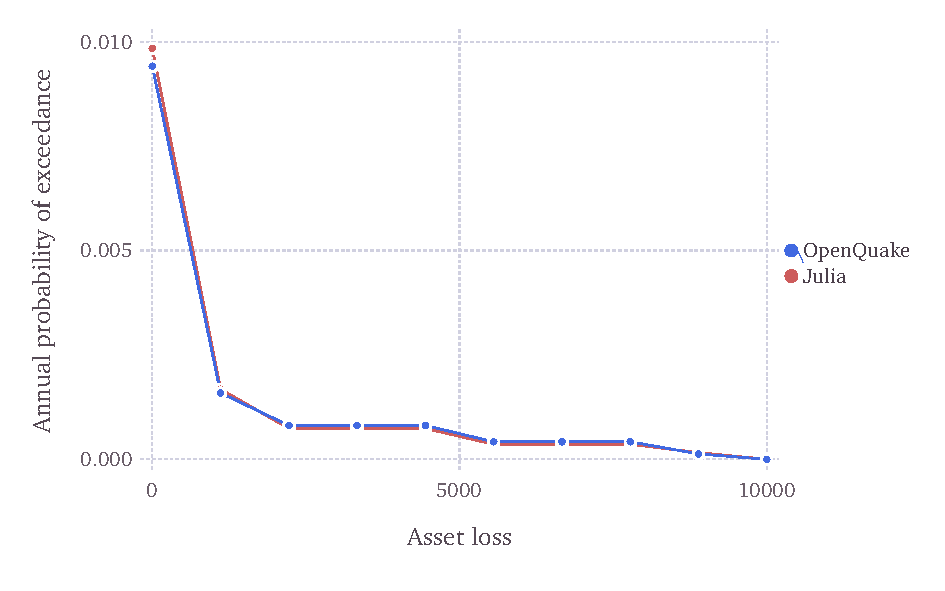
\includegraphics[width=12cm]{qareport/figures/fig-lc-ebr-1g}
\caption{Loss curve comparison for event based risk test case 1g}
\label{fig:lc-ebr-1g}
\end{figure}

The area under the annual loss exceedance curve gives the average annual loss.
\begin{table}[htbp]

\centering
\begin{tabular}{ l r r r }

\hline
\rowcolor{anti-flashwhite}
\bf{Result} & \bf{Julia} & \bf{OpenQuake} & \bf{Difference}\\
\hline
Average loss & 11.17 & 11.23 & 0.53\% \\
\hline
\end{tabular}

\caption{Results for event based risk test case 1g}
\label{tab:result-ebr-1g}
\end{table}
Table \ref{tab:result-ebr-1g} shows the comparison of the OpenQuake result for average annual loss with the expected result.

